% Options for packages loaded elsewhere
\PassOptionsToPackage{unicode}{hyperref}
\PassOptionsToPackage{hyphens}{url}
\PassOptionsToPackage{dvipsnames,svgnames,x11names}{xcolor}
%
\documentclass[
]{article}

\usepackage{amsmath,amssymb}
\usepackage{iftex}
\ifPDFTeX
  \usepackage[T1]{fontenc}
  \usepackage[utf8]{inputenc}
  \usepackage{textcomp} % provide euro and other symbols
\else % if luatex or xetex
  \usepackage{unicode-math}
  \defaultfontfeatures{Scale=MatchLowercase}
  \defaultfontfeatures[\rmfamily]{Ligatures=TeX,Scale=1}
\fi
\usepackage{lmodern}
\ifPDFTeX\else  
    % xetex/luatex font selection
\fi
% Use upquote if available, for straight quotes in verbatim environments
\IfFileExists{upquote.sty}{\usepackage{upquote}}{}
\IfFileExists{microtype.sty}{% use microtype if available
  \usepackage[]{microtype}
  \UseMicrotypeSet[protrusion]{basicmath} % disable protrusion for tt fonts
}{}
\makeatletter
\@ifundefined{KOMAClassName}{% if non-KOMA class
  \IfFileExists{parskip.sty}{%
    \usepackage{parskip}
  }{% else
    \setlength{\parindent}{0pt}
    \setlength{\parskip}{6pt plus 2pt minus 1pt}}
}{% if KOMA class
  \KOMAoptions{parskip=half}}
\makeatother
\usepackage{xcolor}
\setlength{\emergencystretch}{3em} % prevent overfull lines
\setcounter{secnumdepth}{-\maxdimen} % remove section numbering
% Make \paragraph and \subparagraph free-standing
\ifx\paragraph\undefined\else
  \let\oldparagraph\paragraph
  \renewcommand{\paragraph}[1]{\oldparagraph{#1}\mbox{}}
\fi
\ifx\subparagraph\undefined\else
  \let\oldsubparagraph\subparagraph
  \renewcommand{\subparagraph}[1]{\oldsubparagraph{#1}\mbox{}}
\fi

\usepackage{color}
\usepackage{fancyvrb}
\newcommand{\VerbBar}{|}
\newcommand{\VERB}{\Verb[commandchars=\\\{\}]}
\DefineVerbatimEnvironment{Highlighting}{Verbatim}{commandchars=\\\{\}}
% Add ',fontsize=\small' for more characters per line
\usepackage{framed}
\definecolor{shadecolor}{RGB}{241,243,245}
\newenvironment{Shaded}{\begin{snugshade}}{\end{snugshade}}
\newcommand{\AlertTok}[1]{\textcolor[rgb]{0.68,0.00,0.00}{#1}}
\newcommand{\AnnotationTok}[1]{\textcolor[rgb]{0.37,0.37,0.37}{#1}}
\newcommand{\AttributeTok}[1]{\textcolor[rgb]{0.40,0.45,0.13}{#1}}
\newcommand{\BaseNTok}[1]{\textcolor[rgb]{0.68,0.00,0.00}{#1}}
\newcommand{\BuiltInTok}[1]{\textcolor[rgb]{0.00,0.23,0.31}{#1}}
\newcommand{\CharTok}[1]{\textcolor[rgb]{0.13,0.47,0.30}{#1}}
\newcommand{\CommentTok}[1]{\textcolor[rgb]{0.37,0.37,0.37}{#1}}
\newcommand{\CommentVarTok}[1]{\textcolor[rgb]{0.37,0.37,0.37}{\textit{#1}}}
\newcommand{\ConstantTok}[1]{\textcolor[rgb]{0.56,0.35,0.01}{#1}}
\newcommand{\ControlFlowTok}[1]{\textcolor[rgb]{0.00,0.23,0.31}{#1}}
\newcommand{\DataTypeTok}[1]{\textcolor[rgb]{0.68,0.00,0.00}{#1}}
\newcommand{\DecValTok}[1]{\textcolor[rgb]{0.68,0.00,0.00}{#1}}
\newcommand{\DocumentationTok}[1]{\textcolor[rgb]{0.37,0.37,0.37}{\textit{#1}}}
\newcommand{\ErrorTok}[1]{\textcolor[rgb]{0.68,0.00,0.00}{#1}}
\newcommand{\ExtensionTok}[1]{\textcolor[rgb]{0.00,0.23,0.31}{#1}}
\newcommand{\FloatTok}[1]{\textcolor[rgb]{0.68,0.00,0.00}{#1}}
\newcommand{\FunctionTok}[1]{\textcolor[rgb]{0.28,0.35,0.67}{#1}}
\newcommand{\ImportTok}[1]{\textcolor[rgb]{0.00,0.46,0.62}{#1}}
\newcommand{\InformationTok}[1]{\textcolor[rgb]{0.37,0.37,0.37}{#1}}
\newcommand{\KeywordTok}[1]{\textcolor[rgb]{0.00,0.23,0.31}{#1}}
\newcommand{\NormalTok}[1]{\textcolor[rgb]{0.00,0.23,0.31}{#1}}
\newcommand{\OperatorTok}[1]{\textcolor[rgb]{0.37,0.37,0.37}{#1}}
\newcommand{\OtherTok}[1]{\textcolor[rgb]{0.00,0.23,0.31}{#1}}
\newcommand{\PreprocessorTok}[1]{\textcolor[rgb]{0.68,0.00,0.00}{#1}}
\newcommand{\RegionMarkerTok}[1]{\textcolor[rgb]{0.00,0.23,0.31}{#1}}
\newcommand{\SpecialCharTok}[1]{\textcolor[rgb]{0.37,0.37,0.37}{#1}}
\newcommand{\SpecialStringTok}[1]{\textcolor[rgb]{0.13,0.47,0.30}{#1}}
\newcommand{\StringTok}[1]{\textcolor[rgb]{0.13,0.47,0.30}{#1}}
\newcommand{\VariableTok}[1]{\textcolor[rgb]{0.07,0.07,0.07}{#1}}
\newcommand{\VerbatimStringTok}[1]{\textcolor[rgb]{0.13,0.47,0.30}{#1}}
\newcommand{\WarningTok}[1]{\textcolor[rgb]{0.37,0.37,0.37}{\textit{#1}}}

\providecommand{\tightlist}{%
  \setlength{\itemsep}{0pt}\setlength{\parskip}{0pt}}\usepackage{longtable,booktabs,array}
\usepackage{calc} % for calculating minipage widths
% Correct order of tables after \paragraph or \subparagraph
\usepackage{etoolbox}
\makeatletter
\patchcmd\longtable{\par}{\if@noskipsec\mbox{}\fi\par}{}{}
\makeatother
% Allow footnotes in longtable head/foot
\IfFileExists{footnotehyper.sty}{\usepackage{footnotehyper}}{\usepackage{footnote}}
\makesavenoteenv{longtable}
\usepackage{graphicx}
\makeatletter
\def\maxwidth{\ifdim\Gin@nat@width>\linewidth\linewidth\else\Gin@nat@width\fi}
\def\maxheight{\ifdim\Gin@nat@height>\textheight\textheight\else\Gin@nat@height\fi}
\makeatother
% Scale images if necessary, so that they will not overflow the page
% margins by default, and it is still possible to overwrite the defaults
% using explicit options in \includegraphics[width, height, ...]{}
\setkeys{Gin}{width=\maxwidth,height=\maxheight,keepaspectratio}
% Set default figure placement to htbp
\makeatletter
\def\fps@figure{htbp}
\makeatother

\usepackage{booktabs}
\usepackage{longtable}
\usepackage{array}
\usepackage{multirow}
\usepackage{wrapfig}
\usepackage{float}
\usepackage{colortbl}
\usepackage{pdflscape}
\usepackage{tabu}
\usepackage{threeparttable}
\usepackage{threeparttablex}
\usepackage[normalem]{ulem}
\usepackage{makecell}
\usepackage{xcolor}
\makeatletter
\@ifpackageloaded{caption}{}{\usepackage{caption}}
\AtBeginDocument{%
\ifdefined\contentsname
  \renewcommand*\contentsname{Table of contents}
\else
  \newcommand\contentsname{Table of contents}
\fi
\ifdefined\listfigurename
  \renewcommand*\listfigurename{List of Figures}
\else
  \newcommand\listfigurename{List of Figures}
\fi
\ifdefined\listtablename
  \renewcommand*\listtablename{List of Tables}
\else
  \newcommand\listtablename{List of Tables}
\fi
\ifdefined\figurename
  \renewcommand*\figurename{Figure}
\else
  \newcommand\figurename{Figure}
\fi
\ifdefined\tablename
  \renewcommand*\tablename{Table}
\else
  \newcommand\tablename{Table}
\fi
}
\@ifpackageloaded{float}{}{\usepackage{float}}
\floatstyle{ruled}
\@ifundefined{c@chapter}{\newfloat{codelisting}{h}{lop}}{\newfloat{codelisting}{h}{lop}[chapter]}
\floatname{codelisting}{Listing}
\newcommand*\listoflistings{\listof{codelisting}{List of Listings}}
\makeatother
\makeatletter
\makeatother
\makeatletter
\@ifpackageloaded{caption}{}{\usepackage{caption}}
\@ifpackageloaded{subcaption}{}{\usepackage{subcaption}}
\makeatother
\ifLuaTeX
  \usepackage{selnolig}  % disable illegal ligatures
\fi
\usepackage{bookmark}

\IfFileExists{xurl.sty}{\usepackage{xurl}}{} % add URL line breaks if available
\urlstyle{same} % disable monospaced font for URLs
\hypersetup{
  pdftitle={Evaluación Taller Intermedio OHWe 2025},
  pdfauthor={Dr.~Juan Carlos Saavedra-Nievas},
  colorlinks=true,
  linkcolor={blue},
  filecolor={Maroon},
  citecolor={Blue},
  urlcolor={Blue},
  pdfcreator={LaTeX via pandoc}}

\title{Evaluación Taller Intermedio OHWe 2025}
\author{Dr.~Juan Carlos Saavedra-Nievas}
\date{2025-10-18}

\begin{document}
\maketitle

\renewcommand*\contentsname{Table of contents}
{
\hypersetup{linkcolor=}
\setcounter{tocdepth}{3}
\tableofcontents
}
\begin{center}

\includegraphics[width=1.625in,height=\textheight]{OHWe.png}
\end{center}

\subsection{Fuente de datos}\label{fuente-de-datos}

Para ilustrar la manipulación de datos temporales y espaciales se
utilizará la información proveniente del producto \emph{Global Ocean
Physics Analysis and Forecast.}

\url{https://data.marine.copernicus.eu/es/product/GLOBAL_ANALYSISFORECAST_PHY_001_024/}

De Copernicus (\url{https://marine.copernicus.eu/}).

\begin{figure}[H]

{\centering 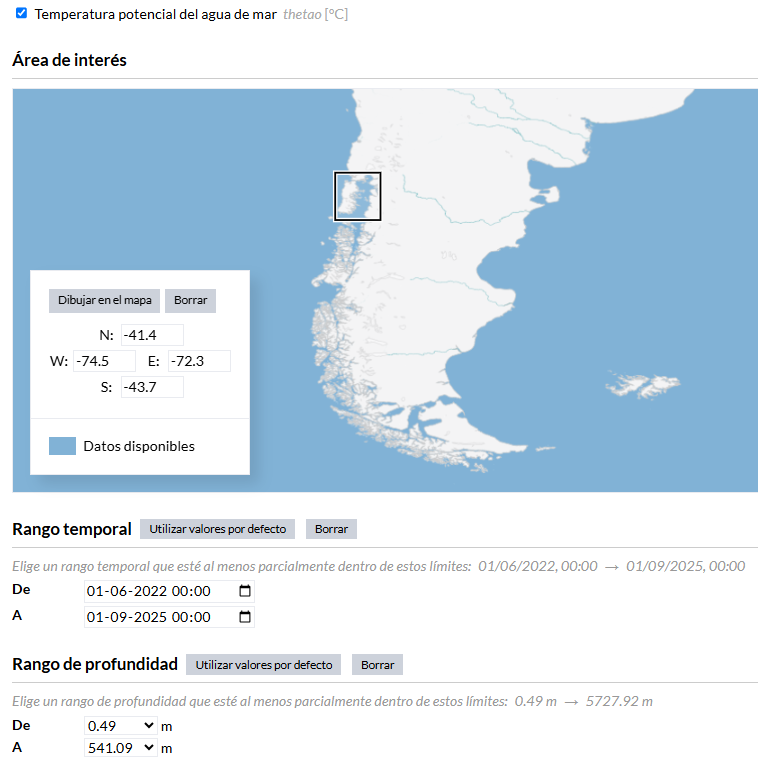
\includegraphics[width=6.77083in,height=\textheight]{DataCopernicus.png}

}

\caption{\textbf{Figura 1}. Obtención de datos desde Copernicus}

\end{figure}%

El archivo netCDF contiene datos mensuales de la temperatura potencial
del mar para la zona de la Isla Grande de Chiloe, Chile (\textbf{Figura
1}). El periodo abarca desde junio del 2022 a septiembre de 2025, en
profundidades entre los 500 metros y la superficie del mar (a medio
metro).

\subsection{\texorpdfstring{Importación a
\texttt{RStudio}}{Importación a RStudio}}\label{importaciuxf3n-a-rstudio}

\subsubsection{\texorpdfstring{Importacion con las librerias
\textbf{\texttt{ncdf4}} y
\textbf{\texttt{satin}}}{Importacion con las librerias ncdf4 y satin}}\label{importacion-con-las-librerias-ncdf4-y-satin}

La importación de datos puede ser realizada con la función
\texttt{nc\_open()} el paquete \textbf{\texttt{ncdf4}} o con la función
\texttt{read.cmems()} del paquete \textbf{\texttt{satin}} disponible en
la cuenta de GitHub \textbf{\emph{hvillalo}}.

\begin{Shaded}
\begin{Highlighting}[]
\NormalTok{dat\_temp1 }\OtherTok{\textless{}{-}} \FunctionTok{nc\_open}\NormalTok{(}\StringTok{"./Datos/cmems\_mod\_glo\_phy{-}thetao\_anfc\_0.083deg\_P1M{-}m\_1760545237347.nc"}\NormalTok{)}
\NormalTok{dat\_temp2 }\OtherTok{\textless{}{-}} \FunctionTok{read.cmems}\NormalTok{(}\StringTok{"./Datos/cmems\_mod\_glo\_phy{-}thetao\_anfc\_0.083deg\_P1M{-}m\_1760545237347.nc"}\NormalTok{)}
\end{Highlighting}
\end{Shaded}

La información global del archivo netCDF, importado con la función
\texttt{read.cmems()}, se presenta a continuación:

\begin{Shaded}
\begin{Highlighting}[]
\FunctionTok{print.satin\_mod}\NormalTok{(dat\_temp2)}
\end{Highlighting}
\end{Shaded}

\begin{verbatim}
Object of class satin

 Title: thetao 
 Long name: Temperature 
 Name: thetao 
 Units: degrees_C 
 Temporal range: monthly 
 Spatial resolution: 9.3 km 

Data dimensions:
  Lat   Lon  Time Depth 
   28    27    40    32 

Data ranges:
          lon       lat   thetao     period      depth
min -74.49999 -43.66667  4.97568 2022-06-01   0.494025
max -72.33333 -41.41667 18.11768 2025-09-01 541.088928
\end{verbatim}

Podemos ver que tenemos datos mensuales de temperatura en °C, con una
resolución espacial de 9.3 km. En total son 40 meses (jun-2022 a
sep-2025) y 32 niveles de profundidad diferentes (entre 0.5 y 541
metros).

Para generar una tabla con los datos de posición, temporales y de
profundidad utilizamos el objeto \texttt{dat.temp2} clase
\textbf{\texttt{satin}} mediante la función \texttt{formatXTP}
modificada para obtener todas las capas temporales y de profundidad.

\begin{Shaded}
\begin{Highlighting}[]
\NormalTok{sst\_stn }\OtherTok{\textless{}{-}} \FunctionTok{extractPts}\NormalTok{(}\AttributeTok{X =}\NormalTok{ dat\_temp2, }\AttributeTok{points =} \FunctionTok{expand.grid}\NormalTok{(}\AttributeTok{x=}\NormalTok{dat\_temp2}\SpecialCharTok{@}\NormalTok{lon, }\AttributeTok{y=}\NormalTok{dat\_temp2}\SpecialCharTok{@}\NormalTok{lat))}
\NormalTok{dt\_stn }\OtherTok{\textless{}{-}} \FunctionTok{formatXTP}\NormalTok{(sst\_stn)}
\end{Highlighting}
\end{Shaded}

La vista de los 10 primeros registros de datos importados se presenta en
la siguiente tabla.

\begin{longtable}[]{@{}
  >{\raggedright\arraybackslash}p{(\columnwidth - 18\tabcolsep) * \real{0.1410}}
  >{\raggedleft\arraybackslash}p{(\columnwidth - 18\tabcolsep) * \real{0.1154}}
  >{\raggedright\arraybackslash}p{(\columnwidth - 18\tabcolsep) * \real{0.0385}}
  >{\raggedleft\arraybackslash}p{(\columnwidth - 18\tabcolsep) * \real{0.0385}}
  >{\raggedleft\arraybackslash}p{(\columnwidth - 18\tabcolsep) * \real{0.1282}}
  >{\raggedleft\arraybackslash}p{(\columnwidth - 18\tabcolsep) * \real{0.1282}}
  >{\raggedleft\arraybackslash}p{(\columnwidth - 18\tabcolsep) * \real{0.0385}}
  >{\raggedleft\arraybackslash}p{(\columnwidth - 18\tabcolsep) * \real{0.1282}}
  >{\raggedleft\arraybackslash}p{(\columnwidth - 18\tabcolsep) * \real{0.1282}}
  >{\raggedleft\arraybackslash}p{(\columnwidth - 18\tabcolsep) * \real{0.1154}}@{}}
\caption{\textbf{Tabla 1.} Vista primeros 10 registros de datos
importados (n= 967.680)}\tabularnewline
\toprule\noalign{}
\begin{minipage}[b]{\linewidth}\raggedright
Time
\end{minipage} & \begin{minipage}[b]{\linewidth}\raggedleft
Depth
\end{minipage} & \begin{minipage}[b]{\linewidth}\raggedright
tp
\end{minipage} & \begin{minipage}[b]{\linewidth}\raggedleft
id
\end{minipage} & \begin{minipage}[b]{\linewidth}\raggedleft
x
\end{minipage} & \begin{minipage}[b]{\linewidth}\raggedleft
y
\end{minipage} & \begin{minipage}[b]{\linewidth}\raggedleft
d
\end{minipage} & \begin{minipage}[b]{\linewidth}\raggedleft
lon
\end{minipage} & \begin{minipage}[b]{\linewidth}\raggedleft
lat
\end{minipage} & \begin{minipage}[b]{\linewidth}\raggedleft
sst
\end{minipage} \\
\midrule\noalign{}
\endfirsthead
\toprule\noalign{}
\begin{minipage}[b]{\linewidth}\raggedright
Time
\end{minipage} & \begin{minipage}[b]{\linewidth}\raggedleft
Depth
\end{minipage} & \begin{minipage}[b]{\linewidth}\raggedright
tp
\end{minipage} & \begin{minipage}[b]{\linewidth}\raggedleft
id
\end{minipage} & \begin{minipage}[b]{\linewidth}\raggedleft
x
\end{minipage} & \begin{minipage}[b]{\linewidth}\raggedleft
y
\end{minipage} & \begin{minipage}[b]{\linewidth}\raggedleft
d
\end{minipage} & \begin{minipage}[b]{\linewidth}\raggedleft
lon
\end{minipage} & \begin{minipage}[b]{\linewidth}\raggedleft
lat
\end{minipage} & \begin{minipage}[b]{\linewidth}\raggedleft
sst
\end{minipage} \\
\midrule\noalign{}
\endhead
\bottomrule\noalign{}
\endlastfoot
2022-06-01 & 0.494025 & p1 & 1 & -74.49999 & -43.66667 & 0 & -74.49999 &
-43.66667 & 9.890773 \\
2022-06-01 & 0.494025 & p1 & 2 & -74.41666 & -43.66667 & 0 & -74.41666 &
-43.66667 & 9.932520 \\
2022-06-01 & 0.494025 & p1 & 3 & -74.33333 & -43.66667 & 0 & -74.33333 &
-43.66667 & 9.984539 \\
2022-06-01 & 0.494025 & p1 & 4 & -74.24999 & -43.66667 & 0 & -74.24999 &
-43.66667 & 9.969974 \\
2022-06-01 & 0.494025 & p1 & 5 & -74.16666 & -43.66667 & 0 & -74.16666 &
-43.66667 & 9.904797 \\
2022-06-01 & 0.494025 & p1 & 6 & -74.08333 & -43.66667 & 0 & -74.08333 &
-43.66667 & 9.823667 \\
\end{longtable}

El resumen del total de capas y posiciones se presenta en la siguiente
tabla.

\begin{longtable}[]{@{}
  >{\raggedleft\arraybackslash}p{(\columnwidth - 22\tabcolsep) * \real{0.0753}}
  >{\raggedleft\arraybackslash}p{(\columnwidth - 22\tabcolsep) * \real{0.0860}}
  >{\raggedleft\arraybackslash}p{(\columnwidth - 22\tabcolsep) * \real{0.0430}}
  >{\raggedleft\arraybackslash}p{(\columnwidth - 22\tabcolsep) * \real{0.0430}}
  >{\raggedleft\arraybackslash}p{(\columnwidth - 22\tabcolsep) * \real{0.0860}}
  >{\raggedleft\arraybackslash}p{(\columnwidth - 22\tabcolsep) * \real{0.0968}}
  >{\raggedleft\arraybackslash}p{(\columnwidth - 22\tabcolsep) * \real{0.0968}}
  >{\raggedleft\arraybackslash}p{(\columnwidth - 22\tabcolsep) * \real{0.0968}}
  >{\raggedleft\arraybackslash}p{(\columnwidth - 22\tabcolsep) * \real{0.0968}}
  >{\raggedleft\arraybackslash}p{(\columnwidth - 22\tabcolsep) * \real{0.0860}}
  >{\raggedleft\arraybackslash}p{(\columnwidth - 22\tabcolsep) * \real{0.0968}}
  >{\raggedleft\arraybackslash}p{(\columnwidth - 22\tabcolsep) * \real{0.0968}}@{}}
\caption{\textbf{Tabla 2.} Resumen datos importados}\tabularnewline
\toprule\noalign{}
\begin{minipage}[b]{\linewidth}\raggedleft
Time\_n
\end{minipage} & \begin{minipage}[b]{\linewidth}\raggedleft
Depth\_n
\end{minipage} & \begin{minipage}[b]{\linewidth}\raggedleft
x\_n
\end{minipage} & \begin{minipage}[b]{\linewidth}\raggedleft
y\_n
\end{minipage} & \begin{minipage}[b]{\linewidth}\raggedleft
min
\end{minipage} & \begin{minipage}[b]{\linewidth}\raggedleft
max
\end{minipage} & \begin{minipage}[b]{\linewidth}\raggedleft
mean
\end{minipage} & \begin{minipage}[b]{\linewidth}\raggedleft
median
\end{minipage} & \begin{minipage}[b]{\linewidth}\raggedleft
q25
\end{minipage} & \begin{minipage}[b]{\linewidth}\raggedleft
q75
\end{minipage} & \begin{minipage}[b]{\linewidth}\raggedleft
sd
\end{minipage} & \begin{minipage}[b]{\linewidth}\raggedleft
riq
\end{minipage} \\
\midrule\noalign{}
\endfirsthead
\toprule\noalign{}
\begin{minipage}[b]{\linewidth}\raggedleft
Time\_n
\end{minipage} & \begin{minipage}[b]{\linewidth}\raggedleft
Depth\_n
\end{minipage} & \begin{minipage}[b]{\linewidth}\raggedleft
x\_n
\end{minipage} & \begin{minipage}[b]{\linewidth}\raggedleft
y\_n
\end{minipage} & \begin{minipage}[b]{\linewidth}\raggedleft
min
\end{minipage} & \begin{minipage}[b]{\linewidth}\raggedleft
max
\end{minipage} & \begin{minipage}[b]{\linewidth}\raggedleft
mean
\end{minipage} & \begin{minipage}[b]{\linewidth}\raggedleft
median
\end{minipage} & \begin{minipage}[b]{\linewidth}\raggedleft
q25
\end{minipage} & \begin{minipage}[b]{\linewidth}\raggedleft
q75
\end{minipage} & \begin{minipage}[b]{\linewidth}\raggedleft
sd
\end{minipage} & \begin{minipage}[b]{\linewidth}\raggedleft
riq
\end{minipage} \\
\midrule\noalign{}
\endhead
\bottomrule\noalign{}
\endlastfoot
40 & 32 & 27 & 28 & 4.97568 & 18.11768 & 10.87753 & 10.43774 & 9.569804
& 11.8639 & 1.709499 & 2.294091 \\
\end{longtable}

\subsubsection{\texorpdfstring{Importación con la librería
\textbf{\texttt{raster}}}{Importación con la librería raster}}\label{importaciuxf3n-con-la-libreruxeda-raster}

Otra formato de importación es utilizar la función \texttt{brick()} de
la librería \textbf{\texttt{raster}}, que importa los archivos
\texttt{netCDF} en formato \texttt{rasterbrick}. El inconveniente es que
si aparte del tiempo existe otra dimensión (profundidad), solo es
posible importar un nivel de esa capa.

Para solucionar esto, se generó la función \texttt{brick\_mod} que
permite:

\begin{enumerate}
\def\labelenumi{\arabic{enumi}.}
\tightlist
\item
  Importar todas todas las capas temporales para una capa particular de
  profundidad con los argumentos,
  \texttt{dt.time\ =\ TRUE,\ dt.depth\ =\ FALSE,\ level\ =\ 1},
  \texttt{level} indica el número de la capa asociada a la profundidad.

  \begin{itemize}
  \tightlist
  \item
    Para este caso se genera una lista con los objetos
    \emph{``\emph{\texttt{brick.tmp}}''} y
    \emph{``\emph{\texttt{dt.tmp}}''}, el primer objeto contiene el
    \textbf{RasterBrick} para la capa de profundidad elegida (por
    defecto la primera) y el segundo es una tabla con los datos
    temporales, la capa de profundidad elegida, las posiciones y la
    variable de interés.
  \end{itemize}
\item
  Importar todas todas las capas de profundidad para una capa particular
  temporal con los argumentos,
  \texttt{dt.time\ =\ FALSE,\ dt.depth\ =\ TRUE,\ level\ =\ 1},
  \texttt{level} indica el número de la capa asociada a la temporalidad.

  \begin{itemize}
  \tightlist
  \item
    Para este caso se genera una lista con los objetos
    \emph{``\emph{\texttt{brick.dpht}}''} y
    \emph{``\emph{\texttt{dt.dpht}}''}, el primer objeto contiene el
    \textbf{RasterBrick} para cada capa de temporalidad elegida (por
    defecto la primera) y el segundo es una tabla con los datos de
    profundidad, la capa temporal elegida, las posiciones y la variable
    de interés.
  \end{itemize}
\item
  Importar todas todas las capas temporales y de profundidad con los
  argumentos, \texttt{dt.time\ =\ TRUE,\ dt.depth\ =\ TRUE}, el
  argumento \texttt{level} no es utilizado.

  \begin{itemize}
  \tightlist
  \item
    Para este caso se genera una lista con los objetos
    \emph{``\emph{\texttt{brick.tmp}}''} y
    \emph{``\emph{\texttt{dt.td}}''}, el primer objeto contiene los
    \textbf{RasterBrick} para cada capa de profundidad y el segundo es
    una tabla con los datos temporales, la profundidad, las posiciones y
    la variable de interés.
  \end{itemize}
\end{enumerate}

\begin{Shaded}
\begin{Highlighting}[]
\NormalTok{path\_sst }\OtherTok{\textless{}{-}} \StringTok{"./Datos/cmems\_mod\_glo\_phy{-}thetao\_anfc\_0.083deg\_P1M{-}m\_1760545237347.nc"}
\NormalTok{sst\_tmp }\OtherTok{\textless{}{-}} \FunctionTok{brick\_mod}\NormalTok{(path\_sst, }\AttributeTok{dt.time =} \ConstantTok{TRUE}\NormalTok{, }\AttributeTok{dt.depth =} \ConstantTok{FALSE}\NormalTok{, }\AttributeTok{level =} \DecValTok{3}\NormalTok{)}
\NormalTok{sst\_dph }\OtherTok{\textless{}{-}} \FunctionTok{brick\_mod}\NormalTok{(path\_sst, }\AttributeTok{dt.time =} \ConstantTok{FALSE}\NormalTok{, }\AttributeTok{dt.depth =} \ConstantTok{TRUE}\NormalTok{, }\AttributeTok{level =} \DecValTok{4}\NormalTok{)}
\NormalTok{sst\_tmdp }\OtherTok{\textless{}{-}} \FunctionTok{brick\_mod}\NormalTok{(path\_sst, }\AttributeTok{dt.time =} \ConstantTok{TRUE}\NormalTok{, }\AttributeTok{dt.depth =} \ConstantTok{TRUE}\NormalTok{)}
\end{Highlighting}
\end{Shaded}

Los objetos generados en la importación de \texttt{sst\_tmdp} son el
objeto \texttt{brick.tmp} que contiene los atributos de la clase
\textbf{RasterBrick} y \texttt{dt.td} con la tabla de datos temporales,
espaciales (\texttt{lat}, \texttt{lon} y \texttt{depth}) y la variable
de interés.

\begin{Shaded}
\begin{Highlighting}[]
\FunctionTok{names}\NormalTok{(sst\_tmdp)}
\end{Highlighting}
\end{Shaded}

\begin{verbatim}
[1] "brick.tmp" "dt.td"    
\end{verbatim}

Para este caso se tienen tantos objetos \textbf{RasterBrick} como
profundidades se tengan:

\begin{Shaded}
\begin{Highlighting}[]
\FunctionTok{round}\NormalTok{(}\FunctionTok{as.numeric}\NormalTok{(}\FunctionTok{names}\NormalTok{(sst\_tmdp}\SpecialCharTok{$}\NormalTok{brick.tmp)),}\DecValTok{1}\NormalTok{)}
\end{Highlighting}
\end{Shaded}

\begin{verbatim}
 [1]   0.5   1.5   2.6   3.8   5.1   6.4   7.9   9.6  11.4  13.5  15.8  18.5
[13]  21.6  25.2  29.4  34.4  40.3  47.4  55.8  65.8  77.9  92.3 109.7 130.7
[25] 155.9 186.1 222.5 266.0 318.1 380.2 453.9 541.1
\end{verbatim}

Por ultimo la resolución espacial de los datos importados con la función
\texttt{brick\_mod()} es 9.3 km y el resumen del total de capas y
posiciones se presenta en la siguiente tabla.

\begin{longtable}[]{@{}
  >{\raggedleft\arraybackslash}p{(\columnwidth - 22\tabcolsep) * \real{0.0753}}
  >{\raggedleft\arraybackslash}p{(\columnwidth - 22\tabcolsep) * \real{0.0860}}
  >{\raggedleft\arraybackslash}p{(\columnwidth - 22\tabcolsep) * \real{0.0430}}
  >{\raggedleft\arraybackslash}p{(\columnwidth - 22\tabcolsep) * \real{0.0430}}
  >{\raggedleft\arraybackslash}p{(\columnwidth - 22\tabcolsep) * \real{0.0860}}
  >{\raggedleft\arraybackslash}p{(\columnwidth - 22\tabcolsep) * \real{0.0968}}
  >{\raggedleft\arraybackslash}p{(\columnwidth - 22\tabcolsep) * \real{0.0968}}
  >{\raggedleft\arraybackslash}p{(\columnwidth - 22\tabcolsep) * \real{0.0968}}
  >{\raggedleft\arraybackslash}p{(\columnwidth - 22\tabcolsep) * \real{0.0968}}
  >{\raggedleft\arraybackslash}p{(\columnwidth - 22\tabcolsep) * \real{0.0860}}
  >{\raggedleft\arraybackslash}p{(\columnwidth - 22\tabcolsep) * \real{0.0968}}
  >{\raggedleft\arraybackslash}p{(\columnwidth - 22\tabcolsep) * \real{0.0968}}@{}}
\caption{\textbf{Tabla 3}. Resumen datos importados}\tabularnewline
\toprule\noalign{}
\begin{minipage}[b]{\linewidth}\raggedleft
Time\_n
\end{minipage} & \begin{minipage}[b]{\linewidth}\raggedleft
Depth\_n
\end{minipage} & \begin{minipage}[b]{\linewidth}\raggedleft
x\_n
\end{minipage} & \begin{minipage}[b]{\linewidth}\raggedleft
y\_n
\end{minipage} & \begin{minipage}[b]{\linewidth}\raggedleft
min
\end{minipage} & \begin{minipage}[b]{\linewidth}\raggedleft
max
\end{minipage} & \begin{minipage}[b]{\linewidth}\raggedleft
mean
\end{minipage} & \begin{minipage}[b]{\linewidth}\raggedleft
median
\end{minipage} & \begin{minipage}[b]{\linewidth}\raggedleft
q25
\end{minipage} & \begin{minipage}[b]{\linewidth}\raggedleft
q75
\end{minipage} & \begin{minipage}[b]{\linewidth}\raggedleft
sd
\end{minipage} & \begin{minipage}[b]{\linewidth}\raggedleft
riq
\end{minipage} \\
\midrule\noalign{}
\endfirsthead
\toprule\noalign{}
\begin{minipage}[b]{\linewidth}\raggedleft
Time\_n
\end{minipage} & \begin{minipage}[b]{\linewidth}\raggedleft
Depth\_n
\end{minipage} & \begin{minipage}[b]{\linewidth}\raggedleft
x\_n
\end{minipage} & \begin{minipage}[b]{\linewidth}\raggedleft
y\_n
\end{minipage} & \begin{minipage}[b]{\linewidth}\raggedleft
min
\end{minipage} & \begin{minipage}[b]{\linewidth}\raggedleft
max
\end{minipage} & \begin{minipage}[b]{\linewidth}\raggedleft
mean
\end{minipage} & \begin{minipage}[b]{\linewidth}\raggedleft
median
\end{minipage} & \begin{minipage}[b]{\linewidth}\raggedleft
q25
\end{minipage} & \begin{minipage}[b]{\linewidth}\raggedleft
q75
\end{minipage} & \begin{minipage}[b]{\linewidth}\raggedleft
sd
\end{minipage} & \begin{minipage}[b]{\linewidth}\raggedleft
riq
\end{minipage} \\
\midrule\noalign{}
\endhead
\bottomrule\noalign{}
\endlastfoot
40 & 32 & 27 & 28 & 4.97568 & 18.11768 & 10.87753 & 10.43774 & 9.569804
& 11.8639 & 1.709499 & 2.294091 \\
\end{longtable}

\subsection{\texorpdfstring{Gráfica temporal datos importados desde la
librería
\textbf{\texttt{raster}}}{Gráfica temporal datos importados desde la librería raster}}\label{gruxe1fica-temporal-datos-importados-desde-la-libreruxeda-raster}

Construcción de tabla de datos considerando intervalos de profundidad de
aproximadamente 100 metros.

\begin{Shaded}
\begin{Highlighting}[]
\NormalTok{tbl\_catp }\OtherTok{\textless{}{-}}\NormalTok{ sst\_tmdp}\SpecialCharTok{$}\NormalTok{dt.td }\SpecialCharTok{\%\textgreater{}\%} 
  \FunctionTok{mutate}\NormalTok{(}\AttributeTok{Cat\_Depth =} \FunctionTok{cut\_interval}\NormalTok{(Depth, }\DecValTok{5}\NormalTok{)) }\SpecialCharTok{\%\textgreater{}\%} 
  \FunctionTok{group\_by}\NormalTok{(Time, Cat\_Depth) }\SpecialCharTok{\%\textgreater{}\%} 
  \FunctionTok{reframe}\NormalTok{(}
    \AttributeTok{n =} \FunctionTok{n}\NormalTok{(),}
    \AttributeTok{n\_miss =} \FunctionTok{sum}\NormalTok{(}\FunctionTok{is.na}\NormalTok{(sst)),}
    \AttributeTok{p\_complete =} \DecValTok{1}\SpecialCharTok{{-}}\NormalTok{(n\_miss}\SpecialCharTok{/}\NormalTok{n),}
    \AttributeTok{sst=}\FunctionTok{mean}\NormalTok{(sst, }\AttributeTok{na.rm =} \ConstantTok{TRUE}\NormalTok{)) }\SpecialCharTok{\%\textgreater{}\%} 
  \FunctionTok{mutate}\NormalTok{(}\AttributeTok{sst\_mm =} \FunctionTok{c}\NormalTok{(}\FunctionTok{cma}\NormalTok{(sst, }\AttributeTok{order =} \DecValTok{12}\NormalTok{)}\SpecialCharTok{$}\NormalTok{fitted))}
\end{Highlighting}
\end{Shaded}

La vista de los 10 primeros registros de la tabla agrupada por
\texttt{Time} y \texttt{Cat\_Depth} se presenta en la siguiente tabla.

\begin{longtable}[]{@{}
  >{\raggedright\arraybackslash}p{(\columnwidth - 12\tabcolsep) * \real{0.1667}}
  >{\raggedright\arraybackslash}p{(\columnwidth - 12\tabcolsep) * \real{0.1818}}
  >{\raggedleft\arraybackslash}p{(\columnwidth - 12\tabcolsep) * \real{0.0909}}
  >{\raggedleft\arraybackslash}p{(\columnwidth - 12\tabcolsep) * \real{0.1061}}
  >{\raggedleft\arraybackslash}p{(\columnwidth - 12\tabcolsep) * \real{0.1667}}
  >{\raggedleft\arraybackslash}p{(\columnwidth - 12\tabcolsep) * \real{0.1515}}
  >{\raggedleft\arraybackslash}p{(\columnwidth - 12\tabcolsep) * \real{0.1364}}@{}}
\caption{\textbf{Tabla 4.} Vista primeros 10 registros de datos
importados (n= 200)}\tabularnewline
\toprule\noalign{}
\begin{minipage}[b]{\linewidth}\raggedright
Time
\end{minipage} & \begin{minipage}[b]{\linewidth}\raggedright
Cat\_Depth
\end{minipage} & \begin{minipage}[b]{\linewidth}\raggedleft
n
\end{minipage} & \begin{minipage}[b]{\linewidth}\raggedleft
n\_miss
\end{minipage} & \begin{minipage}[b]{\linewidth}\raggedleft
p\_complete
\end{minipage} & \begin{minipage}[b]{\linewidth}\raggedleft
sst
\end{minipage} & \begin{minipage}[b]{\linewidth}\raggedleft
sst\_mm
\end{minipage} \\
\midrule\noalign{}
\endfirsthead
\toprule\noalign{}
\begin{minipage}[b]{\linewidth}\raggedright
Time
\end{minipage} & \begin{minipage}[b]{\linewidth}\raggedright
Cat\_Depth
\end{minipage} & \begin{minipage}[b]{\linewidth}\raggedleft
n
\end{minipage} & \begin{minipage}[b]{\linewidth}\raggedleft
n\_miss
\end{minipage} & \begin{minipage}[b]{\linewidth}\raggedleft
p\_complete
\end{minipage} & \begin{minipage}[b]{\linewidth}\raggedleft
sst
\end{minipage} & \begin{minipage}[b]{\linewidth}\raggedleft
sst\_mm
\end{minipage} \\
\midrule\noalign{}
\endhead
\bottomrule\noalign{}
\endlastfoot
2022-06-01 & {[}0.494,109{]} & 16632 & 8371 & 0.4966931 & 10.034313 &
8.919657 \\
2022-06-01 & (109,217{]} & 3024 & 2431 & 0.1960979 & 8.927974 &
8.892426 \\
2022-06-01 & (217,325{]} & 2268 & 2211 & 0.0251323 & 8.916652 &
8.413693 \\
2022-06-01 & (325,433{]} & 756 & 747 & 0.0119048 & 7.760554 &
8.118268 \\
2022-06-01 & (433,541{]} & 1512 & 1501 & 0.0072751 & 6.508286 &
8.721688 \\
2022-07-01 & {[}0.494,109{]} & 16632 & 8371 & 0.4966931 & 9.532677 &
8.596782 \\
\end{longtable}

La \textbf{Figura 2} presenta la variación promedio de la temperatura
mensual entre junio de 2022 y septiembre de 2025, considerando
intervalos de profundidad de aproximadamente 100 metros. Se observa un
patrón térmico consistente con la estratificación vertical típica de
ambientes marinos, donde la temperatura disminuye progresivamente con la
profundidad. Las variaciones temporales sugieren fluctuaciones
estacionales y posibles eventos de mezcla o intrusiones de masas de agua
más frías en determinados periodos.

\begin{figure}[H]

{\centering 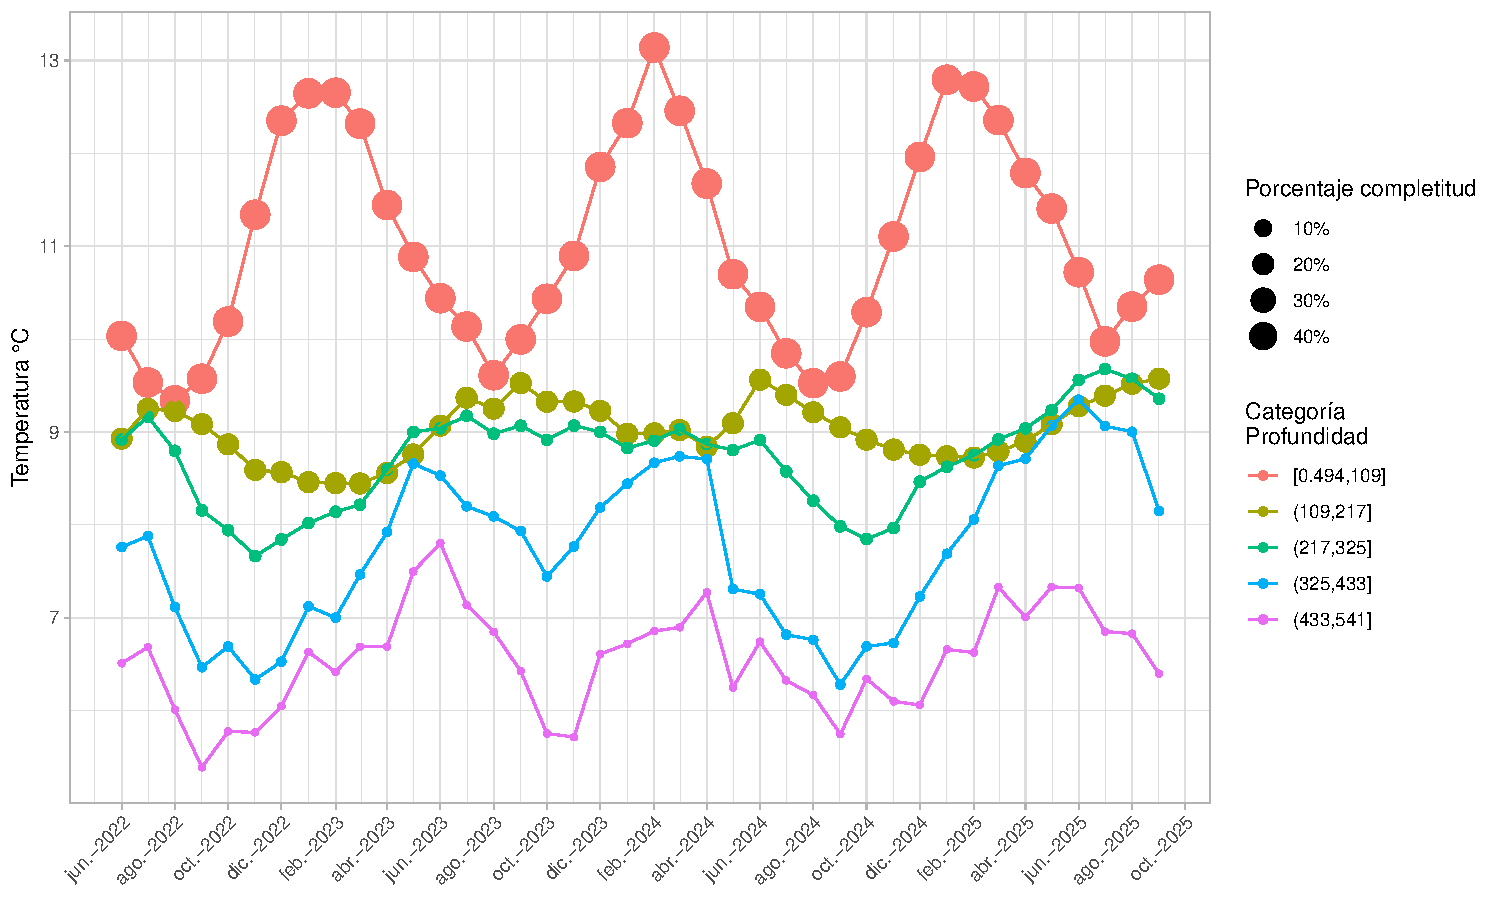
\includegraphics{OHWe_JCSN_2025_files/figure-pdf/unnamed-chunk-13-1.pdf}

}

\caption{\textbf{Figura 2.} Evolución temporal de la temperatura media
para el área de estudio por mes y categoría de profundidad}

\end{figure}%

En la \textbf{Figura 3} se muestran los promedios móviles centrados de
orden 12 aplicados a la serie de temperatura mensual entre junio de 2022
y septiembre de 2025, desagregados por intervalos de profundidad de
aproximadamente 100 metros. El suavizado permite identificar tendencias
de largo plazo en la dinámica térmica, evidenciando posibles ciclos
interanuales y la persistencia de gradientes térmicos verticales en el
período analizado.

\begin{figure}[H]

{\centering 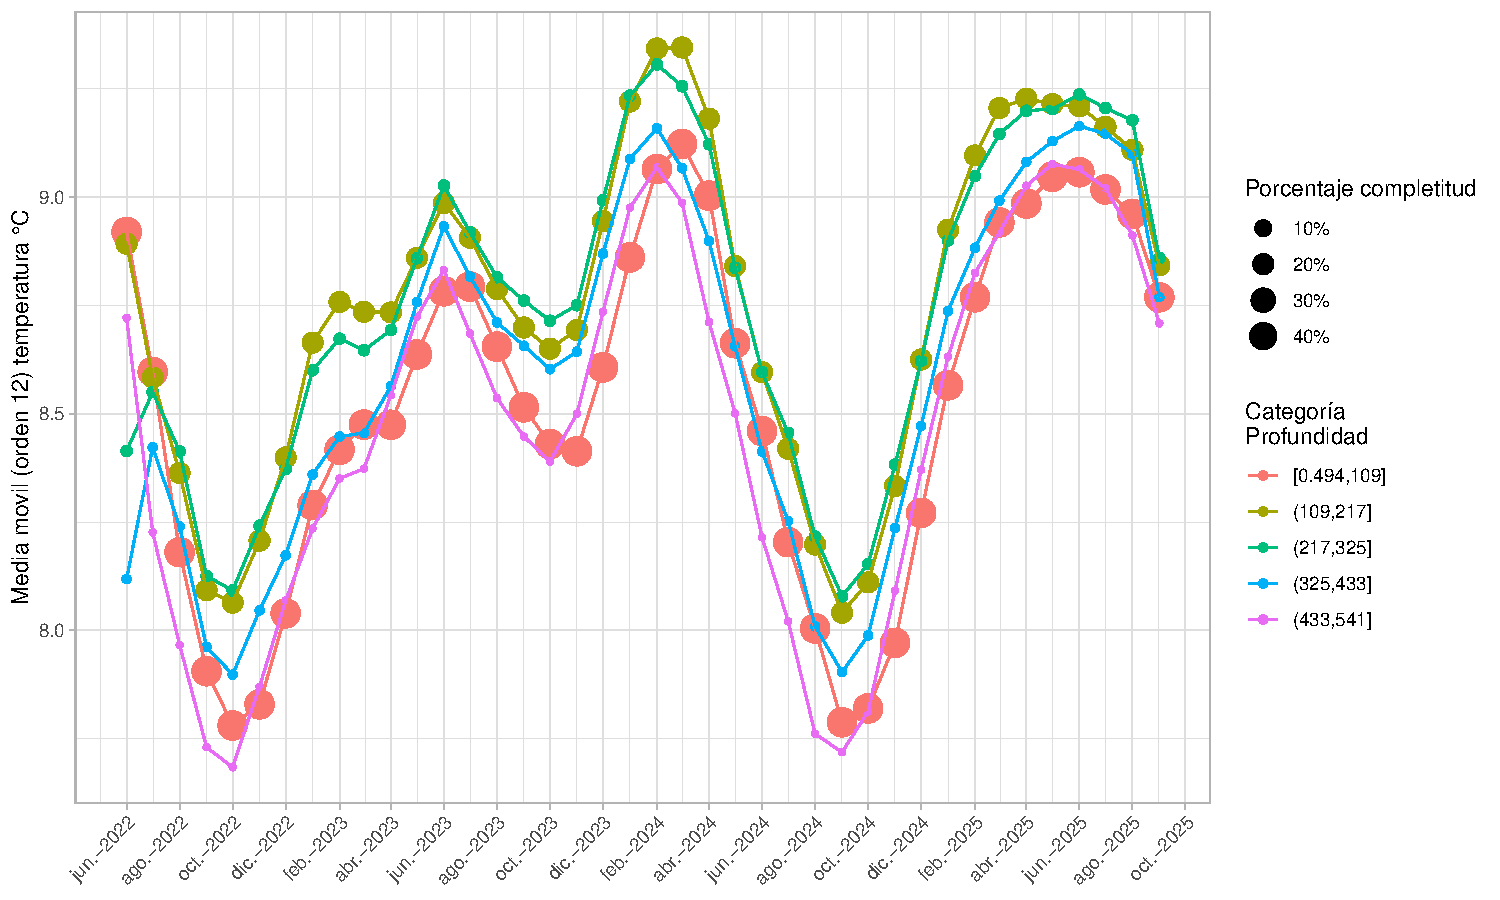
\includegraphics{OHWe_JCSN_2025_files/figure-pdf/unnamed-chunk-14-1.pdf}

}

\caption{\textbf{Figura 3.} Promedios móviles centrados de orden 12 para
el área de estudio por mes y categoría de profundidad}

\end{figure}%

\subsection{\texorpdfstring{Gráfica espacial datos importados desde la
librería
\textbf{\texttt{raster}}}{Gráfica espacial datos importados desde la librería raster}}\label{gruxe1fica-espacial-datos-importados-desde-la-libreruxeda-raster}

La \textbf{Figura 4} compara la temperatura en los meses de agosto y
diciembre de los años 2022 y 2024 para dos categorías de profundidad.
Los resultados revelan diferencias térmicas estacionales marcadas, con
temperaturas superficiales más elevadas en diciembre, asociadas al mayor
calentamiento estival, y valores menores en agosto, correspondientes al
invierno austral. Asimismo, se aprecia una atenuación de las variaciones
térmicas con la profundidad, reflejando una mayor estabilidad de las
masas de agua profundas.

\begin{figure}[H]

{\centering 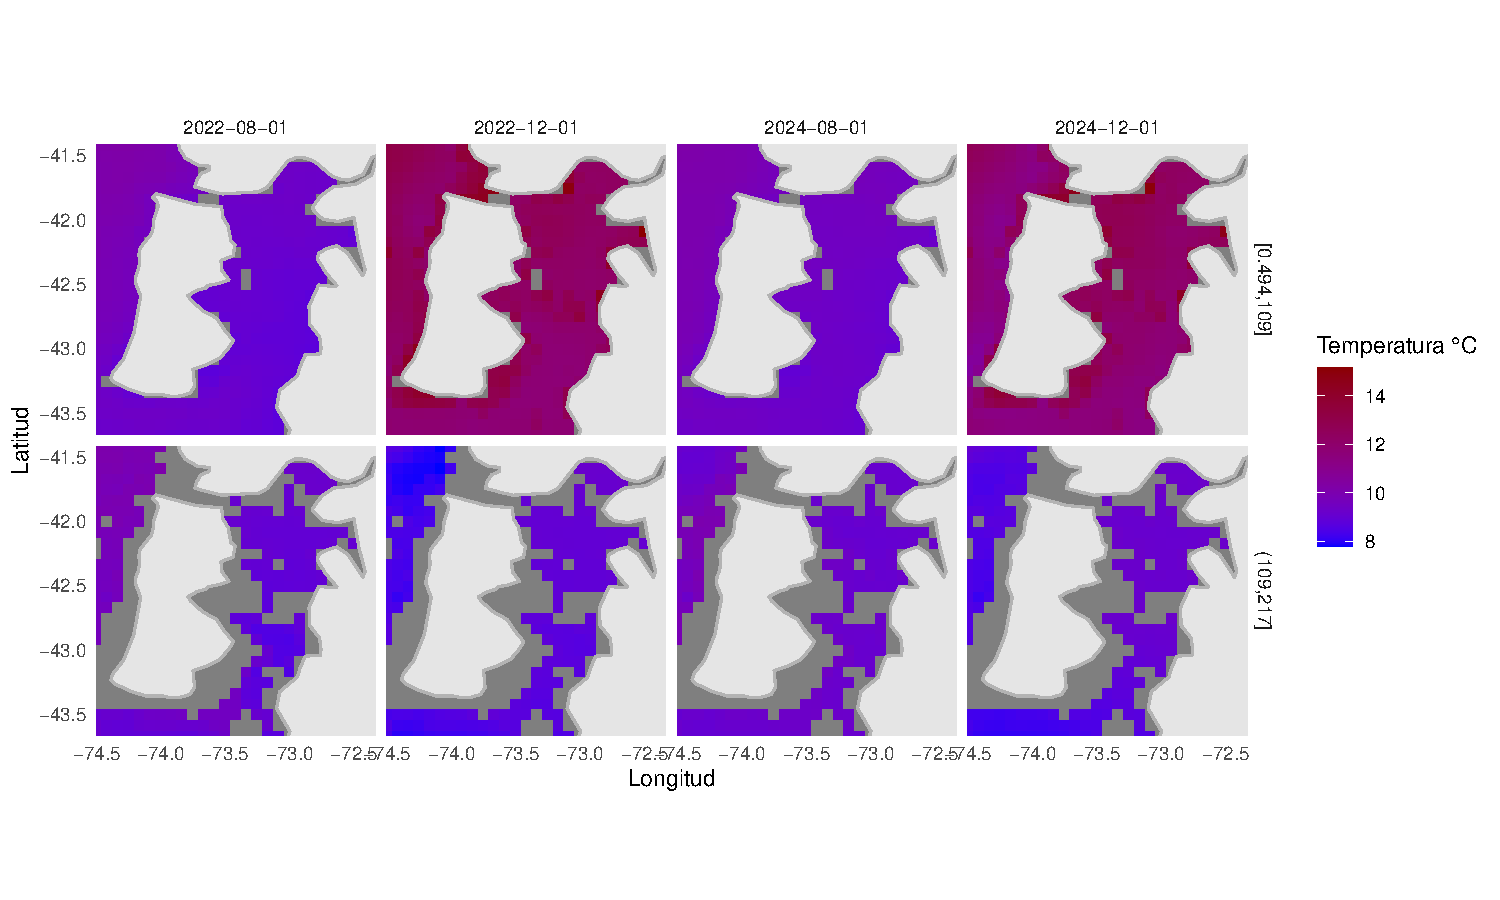
\includegraphics{OHWe_JCSN_2025_files/figure-pdf/unnamed-chunk-15-1.pdf}

}

\caption{\textbf{Figura 4.} Gráficos de la temperatura para las
profundidades entre los 0-100 metros y los 100-200 metros para los meses
de agosto y diciembre de los años 2022 y 2024.}

\end{figure}%



\end{document}
